% !TeX root = main.tex
\label{chap:analysis_requirements}

\section{Yêu cầu chức năng }
Dựa trên mục tiêu và phạm vi, hệ thống FitConnect cần đáp ứng các yêu cầu chức năng chính sau:

\subsection{Quản lý tài khoản và hồ sơ người dùng}
Nhóm tính năng này đảm bảo người dùng tham gia nền tảng và quản lý thông tin cá nhân một cách an toàn và thuận tiện.
\begin{itemize}
    \item \textbf{Đăng ký và Xác thực (FR-01):} Đăng ký tài khoản thông qua Email hoặc Google. Hỗ trợ khôi phục mật khẩu qua Email.
    \item \textbf{Quản lý hồ sơ cá nhân (FR-02):} Xem và cập nhật thông tin cá nhân; quản lý các bài viết đã đăng, sự kiện, thử thách đã tham gia, tập luyện đã tạo,...
\end{itemize}

\subsection{Mạng xã hội cộng đồng}
Nhóm tính năng cộng đồng tạo ra không gian tương tác chuyên biệt cho người yêu thể thao, nơi người dùng có thể trao đổi, chia sẻ các hoạt động, sự kiện, thử thách và tương tác với nhau.
\begin{itemize}
    \item \textbf{Quản lý bài viết (FR-03):} Đăng, chia sẻ, xóa bài viết trên bảng tin cộng đồng. AI hỗ trợ lọc hình ảnh và nội dung không phù hợp khi đăng bài viết.
    \item \textbf{Tương tác xã hội (FR-04):} Thích, bình luận trên bài viết; chia sẻ hoạt động (sự kiện, thử thách) để mọi người cùng tham gia.
    \item \textbf{Báo cáo nội dung vi phạm (FR-05):} Người dùng báo cáo bài viết vi phạm; quản trị viên tiếp nhận và xử lý.
\end{itemize}

\subsection{Sự kiện thể thao (Sport Events)}
Nhóm tính năng sự kiện thể thao cho phép người dùng tổ chức và tham gia các sự kiện thể thao, hướng đến một mục tiêu chung của sự kiện. Hệ thống hỗ trợ cả hai hình thức: hoạt động ngoài trời có theo dõi GPS và hoạt động trong nhà qua video call kết hợp AI.
\begin{itemize}
    \item \textbf{Tổ chức và tham gia sự kiện (FR-06):} Tạo sự kiện (thủ công hoặc AI hỗ trợ tạo) hoặc tham gia sự kiện thể thao (ngoài trời, trong nhà); theo dõi tiến độ cá nhân và chung của sự kiện.
    \item \textbf{Thi đua sự kiện ngoài trời và ghi tiến độ thực (FR-07):} Ghi lộ trình GPS theo thời gian thực; xem quãng đường, thời gian, calo; chia sẻ hoạt động lên cộng đồng.
    \item \textbf{Thi đua sự kiện trong nhà qua Video Call (FR-08):} Video call trực tuyến với mọi người; AI ghi nhận thời gian tham gia hợp lệ; lưu lịch sử buổi tập; chia sẻ hoạt động lên cộng đồng.
    \item \textbf{Chia sẻ và mời tham gia sự kiện (FR-09):} Chia sẻ sự kiện, hoạt động và mời bạn bè, mọi người cùng tham gia.
    \item \textbf{Báo cáo sự kiện vi phạm (FR-10):} Báo cáo sự kiện sai phạm; quản trị viên xử lý.
\end{itemize}

\subsection{Thử thách cộng đồng (Challenges)}
Nhóm tính năng thử thách tập trung vào việc xây dựng kỷ luật cá nhân thông qua các mục tiêu mỗi ngày. Khác với sự kiện thể thao hướng đến mục tiêu chung, thử thách đề cao tiến độ bền bỉ riêng của từng cá nhân theo thời gian.
\begin{itemize}
    \item \textbf{Tạo và tham gia thử thách cộng đồng (FR-11):} Tạo (thủ công hoặc AI hỗ trợ tạo) hoặc tham gia thử thách cộng đồng (ăn uống, tập luyện, ngoài trời).
    \item \textbf{Hoàn thành tiến độ thử thách(FR-12):} Check-in ảnh bữa ăn đối với thử thách ăn uống; Thực hiện tập các bài tập đối với thử thách tập luyện; Đo tiến độ GPS đối với thử thách ngoài trời.
    \item \textbf{Chia sẻ và mời mọi người tham gia (FR-13):} Chia sẻ thử thách, hoạt động và mời bạn bè, mọi người cùng tham gia.
    \item \textbf{Báo cáo vi phạm thử thách (FR-14):} Báo cáo thử thách vi phạm; quản trị viên xử lý.
\end{itemize}

\subsection{Tính toán các chỉ số sức khỏe và gợi ý tập luyện}
Nhóm tính năng này cung cấp bộ công cụ đo lường và theo dõi sức khỏe cá nhân, đồng thời kết hợp trợ lý AI để đưa ra gợi ý tập luyện phù hợp với thể trạng và mục tiêu của từng người dùng.
\begin{itemize}
    \item \textbf{Đo lường các chỉ số sức khỏe (FR-15):} Hệ thống tính toán các chỉ số như BMI, BMR, TDEE và chỉ số liên quan từ thông số cơ thể người dùng nhập.
    \item \textbf{Trợ lý AI phân tích và gợi ý tập luyện (FR-16):} Dựa vào các chỉ số đã tính toán, AI phân tích và gợi ý danh sách các bài tập phù hợp từ danh sách hệ thống bài tập.
    \item \textbf{Theo dõi biểu đồ sức khỏe theo thời gian (FR-17):} Lưu lịch sử chỉ số; hiển thị biểu đồ xu hướng theo thời gian.
\end{itemize}

\subsection{Tập luyện cá nhân}
Nhóm tính năng tập luyện giúp người dùng xây dựng giáo án và duy trì lịch tập cá nhân. Người dùng có thể tự thiết kế bài tập theo nhu cầu hoặc nhận gợi ý tập luyện cá nhân hóa từ AI dựa trên các chỉ số sức khỏe đã đo lường.
\begin{itemize}
    \item \textbf{Tùy biến giáo án thủ công (FR-18):} Dựa vào thiết bị, nhóm cơ muốn tập mà chọn lọc, tùy chỉnh bài tập cho phù hợp.
    \item \textbf{AI gợi ý nhanh bài tập (FR-19):} Nhập mong muốn tập hoặc dựa trên chỉ số sức khỏe, AI gợi ý bộ bài tập phù hợp.
    \item \textbf{Lưu trữ và Lên lịch biểu (FR-20):} Lưu giáo án; xếp lịch tập theo ngày.
    \item \textbf{Rèn luyện thể thao độc lập ngoài trời (FR-21):} Ghi hoạt động ngoài trời (chạy bộ, đạp xe\ldots).
\end{itemize}

\subsection{Kết nối mạng lưới bạn bè}
Nhóm tính năng này xây dựng yếu tố mạng xã hội, giúp người dùng mở rộng mạng lưới quan hệ và duy trì sự gắn kết với những người có chung đam mê thể thao.
\begin{itemize}
    \item \textbf{Theo dõi và Mở rộng mạng lưới (FR-22):} Tìm kiếm, gợi ý, kết bạn hoặc theo dõi thành viên khác.
    \item \textbf{Hoạt động tương tác với bạn bè (FR-23):}  Hoạt động nổi bật (sự kiện, thử thách) của bạn bè hiển thị trên bảng tin.
\end{itemize}

\subsection{Lịch trình cá nhân và thông báo}
Nhóm tính năng này giúp người dùng nắm bắt toàn bộ kế hoạch hoạt động trên một lịch cá nhân thống nhất và nhận được thông báo kịp thời, từ đó duy trì thói quen tập luyện đều đặn.
\begin{itemize}
    \item \textbf{Theo dõi lịch trình hoạt động (FR-24):} Theo dõi lịch sự kiện, thử thách, buổi tập cá nhân mà tôi đã tham gia.
    \item \textbf{Hệ thống thông báo và liên kết bảng tin (FR-25):} Thông báo thời gian thực (nhắc lịch, tương tác bạn bè); có thể đồng bộ hoạt động lên bảng tin.
\end{itemize}

\subsection{Quản trị Hệ thống toàn diện dành cho Quản trị viên}
Phân hệ quản trị cung cấp cho Quản trị viên (Admin) đầy đủ công cụ để giám sát, kiểm soát và vận hành nền tảng một cách hiệu quả, đảm bảo chất lượng nội dung và tính toàn vẹn của dữ liệu hệ thống.
\begin{itemize}
    \item \textbf{Phân tích Dashboard trực quan (FR-26):} Theo dõi, phân tích tình hình hệ thống dựa trên các biểu đồ dashboard.
    \item \textbf{Kiểm soát và Xử lý vi phạm (FR-27):} Xử lý báo cáo; xóa bài viết, sự kiện, thử thách, tài khoản vi phạm.
    \item \textbf{Quản lý toàn diện tài nguyên hệ thống (FR-28):} Truy vấn, chỉnh sửa dữ liệu người dùng, sự kiện, thử thách, danh mục bài tập và cấu hình liên quan.
\end{itemize}

\section{Yêu cầu phi chức năng}
\phantomsection\label{sec:req:nfr_manual}

Bên cạnh yêu cầu chức năng, FitConnect cần đáp ứng các yêu cầu phi chức năng để bảo đảm hiệu năng, an toàn, độ tin cậy và trải nghiệm sử dụng thực tế. Bảng~\ref{tab:nfr_summary} tóm tắt các yêu cầu chính.

% Bảng vừa một trang: dùng table+tabular thay vì longtable để tránh lỗi tách trang
% ``Infinite glue shrinkage found in box being split'' (longtable + \small/\arraystretch).
\begin{table}[H]
\centering
\caption{Tổng hợp yêu cầu phi chức năng hệ thống FitConnect}\label{tab:nfr_summary}
\small
\renewcommand{\arraystretch}{1.15}
\begin{tabular}{|p{3.6cm}|p{10.4cm}|}
\hline
\textbf{Tiêu chí} & \textbf{Yêu cầu chính} \\
\hline
\textbf{Hiệu năng} (Performance) &
Thời gian phản hồi API chính (p95) $\leq$ 2 giây; truy vấn nặng (tìm kiếm/tổng hợp) $\leq$ 3 giây. Hệ thống hỗ trợ tối thiểu 1.000 người dùng đồng thời (theo kịch bản Loader.io) và độ trễ thông báo thời gian thực (WebSocket) trung bình $\leq$ 1 giây. \\
\hline
\textbf{Bảo mật} (Security) &
100\% giao tiếp qua HTTPS; mật khẩu băm Bcrypt (cost factor $\geq$ 10). Access Token hết hạn sau 15 phút, Refresh Token tối đa 7 ngày; khóa tạm 15 phút sau 5 lần đăng nhập sai liên tiếp; rate limiting tối thiểu 100 request/15 phút/IP cho endpoint nhạy cảm; 100\% route quản trị yêu cầu JWT hợp lệ và vai trò Admin. \\
\hline
\textbf{Khả dụng \& Tin cậy} (Availability) &
Mục tiêu uptime dịch vụ $\geq$ 99.5\%/tháng; sao lưu dữ liệu tự động hằng ngày; RPO $\leq$ 24 giờ và RTO $\leq$ 4 giờ khi xảy ra sự cố nghiêm trọng. \\
\hline
\textbf{Mở rộng} (Scalability) &
Hỗ trợ mở rộng ngang tối thiểu 2--3 instance backend sau reverse proxy mà không thay đổi nghiệp vụ; khi tải tăng gấp 2 lần, thời gian phản hồi p95 không vượt quá 3 giây. \\
\hline
\textbf{Tương thích} (Compatibility) &
Responsive cho độ rộng màn hình từ 375px trở lên; hỗ trợ Chrome, Edge, Firefox, Safari ở 2 phiên bản ổn định gần nhất tại thời điểm phát hành. \\
\hline
\textbf{Khả năng sử dụng} (Usability) &
Người dùng mới hoàn thành các tác vụ cốt lõi (đăng ký, tạo bài viết, tham gia sự kiện/thử thách) trong $\leq$ 3 phút mỗi tác vụ; luồng chính không quá 5 thao tác từ màn hình chính. \\
\hline
\textbf{Bảo trì \& Chất lượng mã} (Maintainability) &
Frontend/backend dùng TypeScript và phân tầng rõ ràng; duy trì kiểm thử cho module quan trọng với độ bao phủ tối thiểu 85\% (unit + integration), lint/build phải đạt 100\% trước khi phát hành. \\
\hline
\end{tabular}
\end{table}

\section{Lược đồ Use Case}
Lược đồ Use Case (Tham khảo Hình~\ref{fig:usecase_tong_quat}) trình bày bức tranh tổng thể các chức năng của hệ thống FitConnect dưới góc nhìn của các tác nhân sử dụng. Hai tác nhân chính gồm \textbf{Người dùng (User)} và \textbf{Quản trị viên (Administrator)} với các quyền và phạm vi thao tác khác nhau.

\begin{figure}[H]
    \centering
    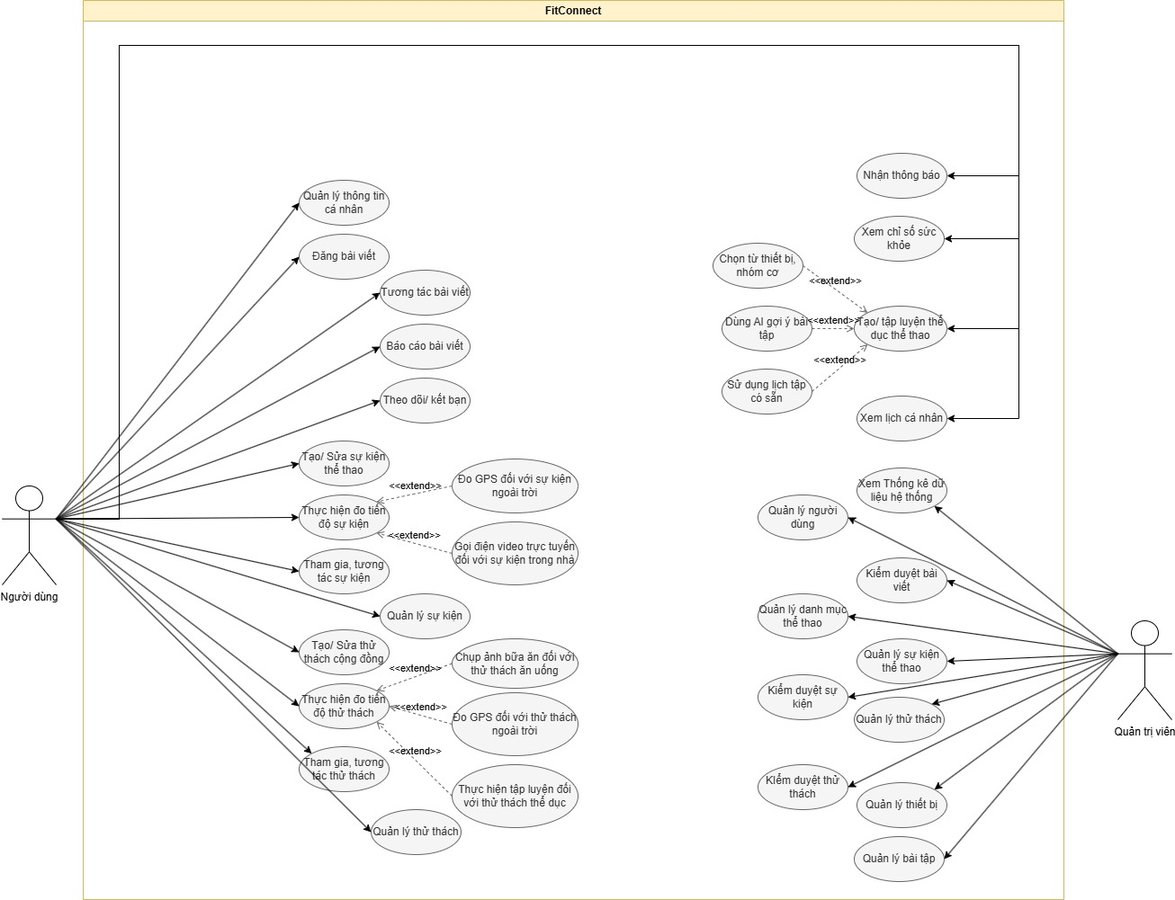
\includegraphics[width=1\textwidth]{Images/IMG/ERD/USECASEDIAGRAMHethong.jpg}
    \vspace{0.5em}
    \caption{Lược đồ Use Case của hệ thống FitConnect}
    \label{fig:usecase_tong_quat}
\end{figure}

Trong lược đồ Use Case, \textbf{Người dùng} có thể quản lý tài khoản, tham gia hoạt động cộng đồng, theo dõi sức khỏe -- tập luyện, đăng ký sự kiện thể thao và tham gia thử thách,... 
\textbf{Quản trị viên} có thể quản trị hệ thống, kiểm duyệt nội dung vi phạm và quản lý các tài nguyên vận hành. Sự phân tách này giúp làm rõ phạm vi chức năng, vai trò của từng tác nhân trong hệ thống.

Đặc tả chi tiết cho 15 trường hợp Use Case được trình bày tại Phụ lục~\ref{sec:usecase_detail} của báo cáo.
